% Reorganização visual do esquema enviado; mesmos polos, campos e limites.
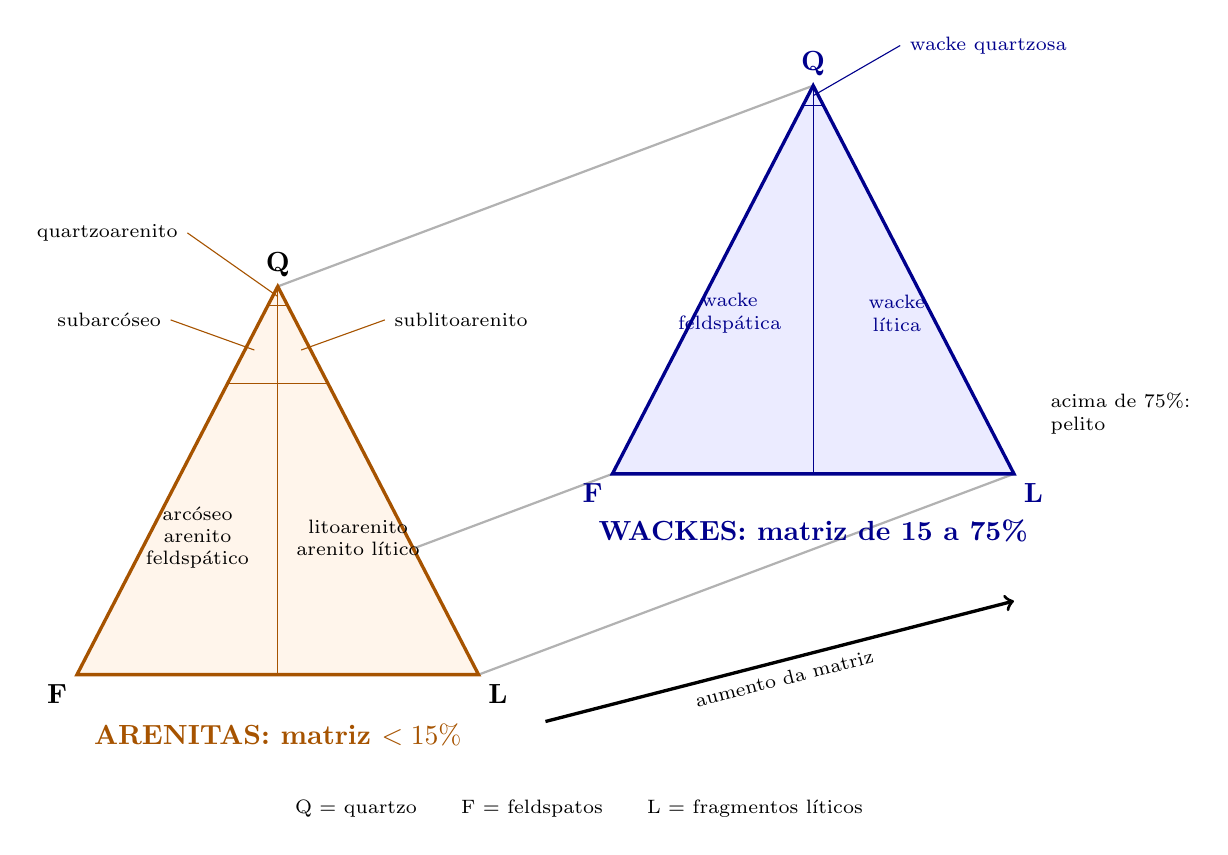
\begin{tikzpicture}[x=0.85cm,y=0.85cm,font=\scriptsize]
\coordinate (Q) at (0,5.8);
\coordinate (F) at (-3,0);
\coordinate (L) at (3,0);
\coordinate (Qb) at (8,8.8);
\coordinate (Fb) at (5,3);
\coordinate (Lb) at (11,3);
\draw[gray!60,thick] (Q)--(Qb) (F)--(Fb) (L)--(Lb);
\path[fill=blue!8] (Qb)--(Fb)--(Lb)--cycle;
\draw[very thick,blue!55!black] (Qb)--(Fb)--(Lb)--cycle;
\draw[blue!55!black] (Qb)--(8,3);
\draw[blue!55!black] (7.85,8.51)--(8.15,8.51);
\path[fill=orange!8] (Q)--(F)--(L)--cycle;
\draw[very thick,orange!65!black] (Q)--(F)--(L)--cycle;
\draw[orange!65!black] (-0.15,5.51)--(0.15,5.51);
\draw[orange!65!black] (-0.75,4.35)--(0.75,4.35);
\draw[orange!65!black] (Q)--(0,0);
\node[above,font=\bfseries] at (Q) {Q};
\node[below left,font=\bfseries] at (F) {F};
\node[below right,font=\bfseries] at (L) {L};
\node[above,font=\bfseries,text=blue!55!black] at (Qb) {Q};
\node[below left,font=\bfseries,text=blue!55!black] at (Fb) {F};
\node[below right,font=\bfseries,text=blue!55!black] at (Lb) {L};
% Rótulos dos campos superiores fora das regiões estreitas.
\draw[orange!65!black] (0,5.65)--(-1.35,6.6);
\node[anchor=east,align=right] at (-1.35,6.6) {quartzoarenito};
\draw[orange!65!black] (-0.35,4.85)--(-1.6,5.3);
\node[anchor=east] at (-1.6,5.3) {subarcóseo};
\draw[orange!65!black] (0.35,4.85)--(1.6,5.3);
\node[anchor=west] at (1.6,5.3) {sublitoarenito};
\node[align=center,text width=1.85cm] at (-1.2,2.05) {arcóseo\\arenito feldspático};
\node[align=center,text width=1.85cm] at (1.2,2.05) {litoarenito\\arenito lítico};
\node[font=\bfseries,text=orange!65!black] at (0,-0.9) {ARENITAS: matriz $<15\%$};
\draw[blue!55!black] (8,8.65)--(9.3,9.4);
\node[anchor=west,text=blue!55!black] at (9.3,9.4) {wacke quartzosa};
\node[align=center,text=blue!55!black] at (6.75,5.4) {wacke\\feldspática};
\node[align=center,text=blue!55!black] at (9.25,5.4) {wacke\\lítica};
\node[font=\bfseries,text=blue!55!black] at (8,2.15) {WACKES: matriz de 15 a 75\%};
\draw[->,very thick] (4,-0.7)--(11,1.1)
 node[midway,below,sloped] {aumento da matriz};
\node[anchor=west,align=left] at (11.4,3.9) {acima de 75\%:\\pelito};
\node[align=center] at (4.5,-2) {Q = quartzo\qquad F = feldspatos\qquad L = fragmentos líticos};
\end{tikzpicture}
